\documentclass[11pt]{article}

\usepackage{threeparttable}
\usepackage{subfig}
\usepackage{pdfpages}
\usepackage{amsfonts,amsthm,amssymb,amsmath}
\usepackage{graphicx,mathrsfs}
\usepackage{multirow}
\usepackage{float}
%\usepackage{tikz}
%\usetikzlibrary{arrows}
\usepackage[hidelinks=true]{hyperref}
\usepackage{natbib}
\bibliographystyle{chicago}
%
% page format
\usepackage[top=0.81in,bottom=0.81in,left=0.81in,right=0.81in%,a4paper
]{geometry}
\linespread{1.3}
\setlength{\parskip}{3.6pt}

%% for cross reference in paper
%\usepackage{hyperref}
%\hypersetup{colorlinks,citecolor=black,filecolor=black,%
%  linkcolor=black,urlcolor=black}

\newtheorem{thm}{Theorem}
\newtheorem{prop}{Proposition}
\newtheorem{assu}{Assumption}
\newtheorem{definition}{Definition}%[section]
\newtheorem{lemma}{Lemma}
\newtheorem{coro}{Corollary}
\newtheorem{example}{Example}
\newtheorem{fact}{Fact}
\newtheorem{conjecture}{Conjecture}
\newtheorem{alg}{Algorithm}
\newtheorem{rem}{Remark}
\newtheorem{fig}{Figure}

\newcommand{\rv}{random variable}
\newcommand{\bE}{\bf E}
\renewcommand{\Box}{\bigboxvoid}
\newcommand{\qeds}{$\qedsymbol $}
\newcommand{\R}{\mathbb{R}}
\newcommand{\Z}{\mathbb{Z}}
\newcommand{\cc}{\mathbb{c}}

 %Natbib setup for author-year style

\title{\textbf{Authors' Reply\\Lagrangian Heuristic for Simultaneous Subsidization and Penalization:\\
Implementations on Rooted Travelling Salesman Games}}
\author{Lindong Liu, Yuqian Zhou, Zikang Li}
\date{}
\begin{document}
\maketitle

\noindent

We would like to thank the Associate Editor for processing our submission efficiently and providing guidance for the revision, and also thank the Referees for the encouraging and detailed comments on the paper.
We have carefully studied all the comments and addressed them in our manuscript.

% In this reply, we summarize several major changes we have made, and then give the specific details.
%
% First, regarding the equality in (4) is replaced to >= inequality in (6), we add a more detailed explanation. Meanwhile we explain that LP(4) is not a restriction of LP(2) in Reply 1 to Referee 1, maybe the term 'restricted LP' on page 7 caused the misunderstanding and we now use 'variant' to replace 'restricted'.
%
% Second, regarding the upper bound $c_u(V)$, we forgot to mention how to obtain the upper bound.
% In fact, all the upper and lower bounds of $c(S)$ are obtained by the Lagrangian relaxation method to keep the consistency and continuity.
%
% Third, regarding the proofs of Theorem 1 and Remark 1, we now add a clarification on the negative cost allocation in Reply 3 to Referee 1 and another clarification on the meaning of "the point-wise maximum of a finite set of straight lines".
%
%
% Fourth, regarding the sub-gradient method, we add a detailed clarification on page 9 including how the initial values of Lagrangian multipiers are given and how they change during the sub-gradient method.
%
%
% Fifth, regarding the symmetry of TSP game and why the TSP game is defined on the complete graph in our manuscript, we make the corresponding explanation in Reply 8 and Reply 6.
%
% Sixth, regarding the Figure 2, we add the definitions of squared points and round points to the legend of the figure and the meaning of curves (a) and (c) in Figure 2 is explained on page 17.
%

Please find below our point-by-point reply to each of the Referees. To facilitate reading, the original comments are in {\it italics}.

%\vspace{10mm}
\newpage

\noindent \textbf{\large Reply to Referee 1}
\\[3mm]
We appreciate your detailed comments.
We have carefully studied the technical concerns you raised, and revised our manuscript accordingly.
One thing we need to mention is that we have changed the notation of coalitions, $s$, to the standard form, $S$, according to the suggestion of  Referee 2.
The main issues raised in your report are addressed as follows:
\\[4mm]
%
%
\noindent \textit{\textbf{Question 1.}
Constraint \# 2 in problem (4). It appears from the next page that the equality can be replaced to $\geq$ inequality in this problem formulation. I would like the authors to expand the discussion of reasons for that being the case as the brief explanation on page 9 does not seem sufficient. Moreover, it looks like a good idea to do it right after introduction of problem (4), since in this case it becomes obvious that (4) is a restriction of (2) and therefore $z_r(w)$ is an upper bound on z(w):}
$$\beta(S) \leq c_l(S) + z \leq c(S) + z$$
$$\beta(V) \geq c_u(V) + z \geq c(S) + z$$
\noindent \textbf{Reply 1.}
Thanks for your question. With regard to the conversion from the equality to the inequality, we have added a more detailed explanation on page 9. And about the second part of this question, maybe the term ``restricted LP" on page 7 caused the misunderstanding and we now use ``variant" to replace ``restricted".

Then we will explain that LP(4) is not a restriction of LP(2) as follows.
Admittedly, this formula $\beta(S) \leq c_l(S) + z \leq c(S) + z$ you wrote is correct, which indicates that $\beta(S) \leq c_l(S) + z$ in LP(4) is a restriction of $\beta(S) \leq c(S) + z$ in LP(2).
% However, we think there are some mistakes in the formula $\beta(V) \geq c_u(U) + z \geq c(s) + z$ you wrote. The first one is, $U$ should be a written error. The second one is, $\beta(V)$ has no direct relation with $z$.
However, we think there is a mistake in the formula $\beta(V) \geq c_u(V) + z \geq c(S) + z$ (maybe it is $c(V)$ rather than $c(S)$) you wrote. That is $\beta(V)$ has no direct relation with $z$.
In fact, according to the cooperative game theory, coalitional stability constraints contain all subcoalitions $S \in \mathbb{S} \setminus \big\{V\big\}$ except the grand coalition $V$.
Thus, the second constraint in LP(4), $\beta(V)=c_u(V)-\omega$, i.e., the budget balance constraint is not a restriction of $\beta(V)=c(V)-\omega$ in LP(2).
Based on the above analysis, LP(4) is just a variant rather than a restriction of LP(2).
% Maybe the 'restricted' word misleads you, so we deleted 'restricted word'.
\\[4mm]
%
%
%
\noindent \textit{\textbf{Question 2.}
When approximate problem (4) is introduced, it is not mentioned which upper bound $c_u(V)$ is used. Probably a discussion of upper bound possibilities will be good here.}
\\[2mm]
\noindent \textbf{Reply 2.}
Thanks a lot for your suggestion. First of all, the upper bound $c_u(V)$ is obtained by the Lagrangian relaxation method, which we forgot to mention. Thank you for reminding us again.
About the second part of this question, there are several specific methods, such as LP-based ones, which can be used to get the bounds for $c(S)$.
In fact, in our manuscript we want to put forward a framework for heuristic algorithms, therefore, the upper and lower bounds of $c(S)$ are both obtained by the Lagrangian relaxation method to keep the consistency and generality. We have added this clarification on page 7.
% In fact, there are specific methods, such as LP-based methods, which can be used to obtain the upper bound $c_u(V)$.
% We have explicitly mentioned this in the paper.
% In order to be consistent with the general methods, we only mentioned a general method, i.e., Lagrangian heuristic to calculate the upper bound $c(V)$.
~\\[4mm]
%
%
%
\noindent \textit{\textbf{Question 3.}
Proof of Theorem 1. This is probably a general question but it also directly affects the proof of Theorem 1. The vector of cost allocation beta is defined to be in $R^v$.
I would like to see some discussion on why some individual cost allocation is allowed to be negative (implying a gain for a player, I guess) and how that is possible with existence of grand coalition. My concern is that beta components in the proof of Theorem 1 can become negative, but, again, I am not sure I understand the meaning of negative cost allocation.}
\\[2mm]
\noindent \textbf{Reply 3.}
%The main contributions are strengthened as explained in the first page of this reply.
Thanks for your question. Yes, when the cost assigned to some player is negative, it can be understood as a gain for the player as you mentioned.
In cooperative game theory, cost allocation does not mean the cost assigned to every player in a cooperative game must be positive. Commonly the vector of cost allocation is defined in $R^v$ (Caprara and Letchford 2010, Schulz and Uhan 2010), and any cost allocation which satisfies the budget balance and coalitional stability constraints we mentioned in the manuscript can make the grand coalition stable (In other words, the grand coalition can exist), even if some components of it are negative.
If the definition of vector of cost allocation in our proof is confined in positive real domain, our result will still hold.
% The beta components in the proof indeed can be negative as you said, that is because the vector of cost allocation which is defined to be in $R^v$ in the proof is mathematically valid.
\\[4mm]
%\textcolor{blue}{
%The main contributions are strengthened as explained in the first page of this reply.
%We have tried our best to shorten the paper.
%There are 25 pages (excluding the reference) in the main part of the revision, while the results are more enriched and compact.
%We hope this is acceptable.}
%\\[4mm]
%
%
\noindent \textit{\textbf{Question 4.}
Proof of Remark 1. I am not able to see ``the point-wise maximum of a finite set of straight lines (hyperplanes, you mean?)" in defining the $z_r(w)$ (19). Please clarity.}
\\[2mm]
\noindent \textbf{Reply 4.}
Thanks for your question. In the objective function of LP(19), $\rho_v \big[ c_u(V)-\omega \big] &- \sum_{S \in \mathbb{S} \setminus \{V\}} \rho_s c_l(S)$ can be seen as a line $l_\rho$ which is related to $\rho$. ``A finite set of straight lines" denotes $l_\rho$ with a finite set of $\rho$.
Therefore, $z_r(w)$, the maximum of the objective function, denotes ``the point-wise maximum of a finite set of straight lines".
We have added this clarification in Proof of Remark 1.
\\[4mm]
%
%
%
\noindent \textit{\textbf{Question 5.}
In the description of the Algorithm 1, how is the initial restricted coalition set is constructed? For example, it is not clear what the first step means means if no initial set is defined. And also, I am not able to see how the initial values of Lagrangian coefficients lambda is constructed and how they change (if they do) during the algorithm. It would be great to add some clarifications.}
~\\[2mm]
\noindent \textbf{Reply 5.}
Thanks for your question. Firstly, the initial restricted coalition set can be selected arbitrarily according to the column generation technique. Commonly we select the set which we think can help to accelerate computation speed. In this case, the restricted coalition set $S'$ is set to be $\{\{1\},\{2\},\ldots, \{v\}\}$, which can also be other forms.
Secondly, about the part of sub-gradient method, we have added the detailed clarification on page 9.
\\[4mm]
%
%
\noindent \textit{\textbf{Question 6.}
The description of the TSP game is somewhat different from one can find in the literature. For example in Tamir (1989) the game was defined on an uncomplete graph, while here the game is defined on the complete graph. This affects all the models presented on page 13 and further. Probably both versions of the game exist, but I would like to understand why the descriptions are different.}
~\\[2mm]
\noindent \textbf{Reply 6.}
Thanks for your question. In Tamir (1989), the author also mentioned that the game was equivalently defined on the complete graph in Potters et al. (1992). Tamir defined the game on an uncomplete graph for the convenience of expression and ease of understanding. In our manuscript, defining TSP game on the complete graph can help us present our idea clearly and conveniently. And we have added the literature, Potters et al. (1992), to the Introduction.
% There is another change mainly for the convenience of presentation.
% For the **, we now define it as ** instead of **.
\\[4mm]
\noindent \textit{\textbf{Question 7.}
Constraint (15): I am not sure why would one keep (15) in such an aggregated format when it is possible to disaggregate it to $x_{ij} \leq \gamma_i$, $x_{ij} \leq \gamma_j$. In terms of LP relaxation disaggregation gives a tighter bound and probably will lead to the improvement to Lagrangian relaxation just as well.}
\\[2mm]
\noindent \textbf{Reply 7.}
Thanks for your suggestion.
The disaggregation format indeed gives a better bound when using LP relaxation.
However, in the Lagrangian relaxation we do not change the integral property of the formulation, i.e., $x_{ij}$ still has to be binary. Considering that the aggregated and disaggregated formats are fully equivalent, thus, the disaggregated format will not lead to the improvement to Lagrangian relaxation.
But for better understanding, we changed the aggregated format to the disaggregated one you mentioned.
\\[4mm]
\noindent \textit{\textbf{Question 8.}
The symmetry of TSP game. I would like to attract the attention of the authors to the Dantzig Fulkerson Johnson (1954) paper, which originated the development of the TSP theory. Most importantly, the authors there also considered a symmetric TSP problem. If the problem is symmetric, one does not need as many binary variables as was introduced by authors. For example, on page 13 $x_{ij}$ exists together with $x_{ji}$ but direction of the travel is not important for symmetric problem therefore it is sufficient to introduce $x_e$ for e being an edge or $x_{ij}$ for $i < j$ only. This is how the TSP problem was introduced in DFJ and this is something that can simplify many notations in this paper. Also, it will be probably a good idea to get rid of $x_{ii}$ variables on page 13 and other optimization problems.}
~\\[2mm]
\noindent \textbf{Reply 8.}
Thanks for your question.
When it comes to a symmetric TSP problem, it is more convenient to introduce $x_e$ or $x_{ij}, i<j$.
However, the player is an important concept in the cooperative game.
We have to express every single node in the TSP game.
If we only use $x_e$ or $x_{ij}, i<j$ to stand for the edge in the TSP game, the notation $\gamma^{S}_j$ used in the rooted TSP game cannot be represented. We have to introduce other notations to represent every single node, which is obviously troublesome.
Thus, we use the expression $x_{ij}, i,j \in N$ in our manuscript.
\\[4mm]
\noindent \textit{\textbf{Question 9.}
I am a bit confused by Figure 2. Does it represent 4 different games? What exactly is on y axis and x axis, Penalty and Subsidy on y and x axis for all 4 figures? I suggest to add definitions of squared points and round points to the legend of the figure. Why is it that one figure gets two points and another gets 6 and they are evaluated at different levels of subsidy?}
~\\[2mm]
\noindent \textbf{Reply 9.}
Thanks for your suggestions. Figure 2 presents four representations of the curves of Lagrangian SPFs. X axis and y axis represent subsidy and penalty respectively for all 4 subfigures. We have added the definitions of squared points and round points to the legend of the figure.
\begin{figure}[H]
\centering
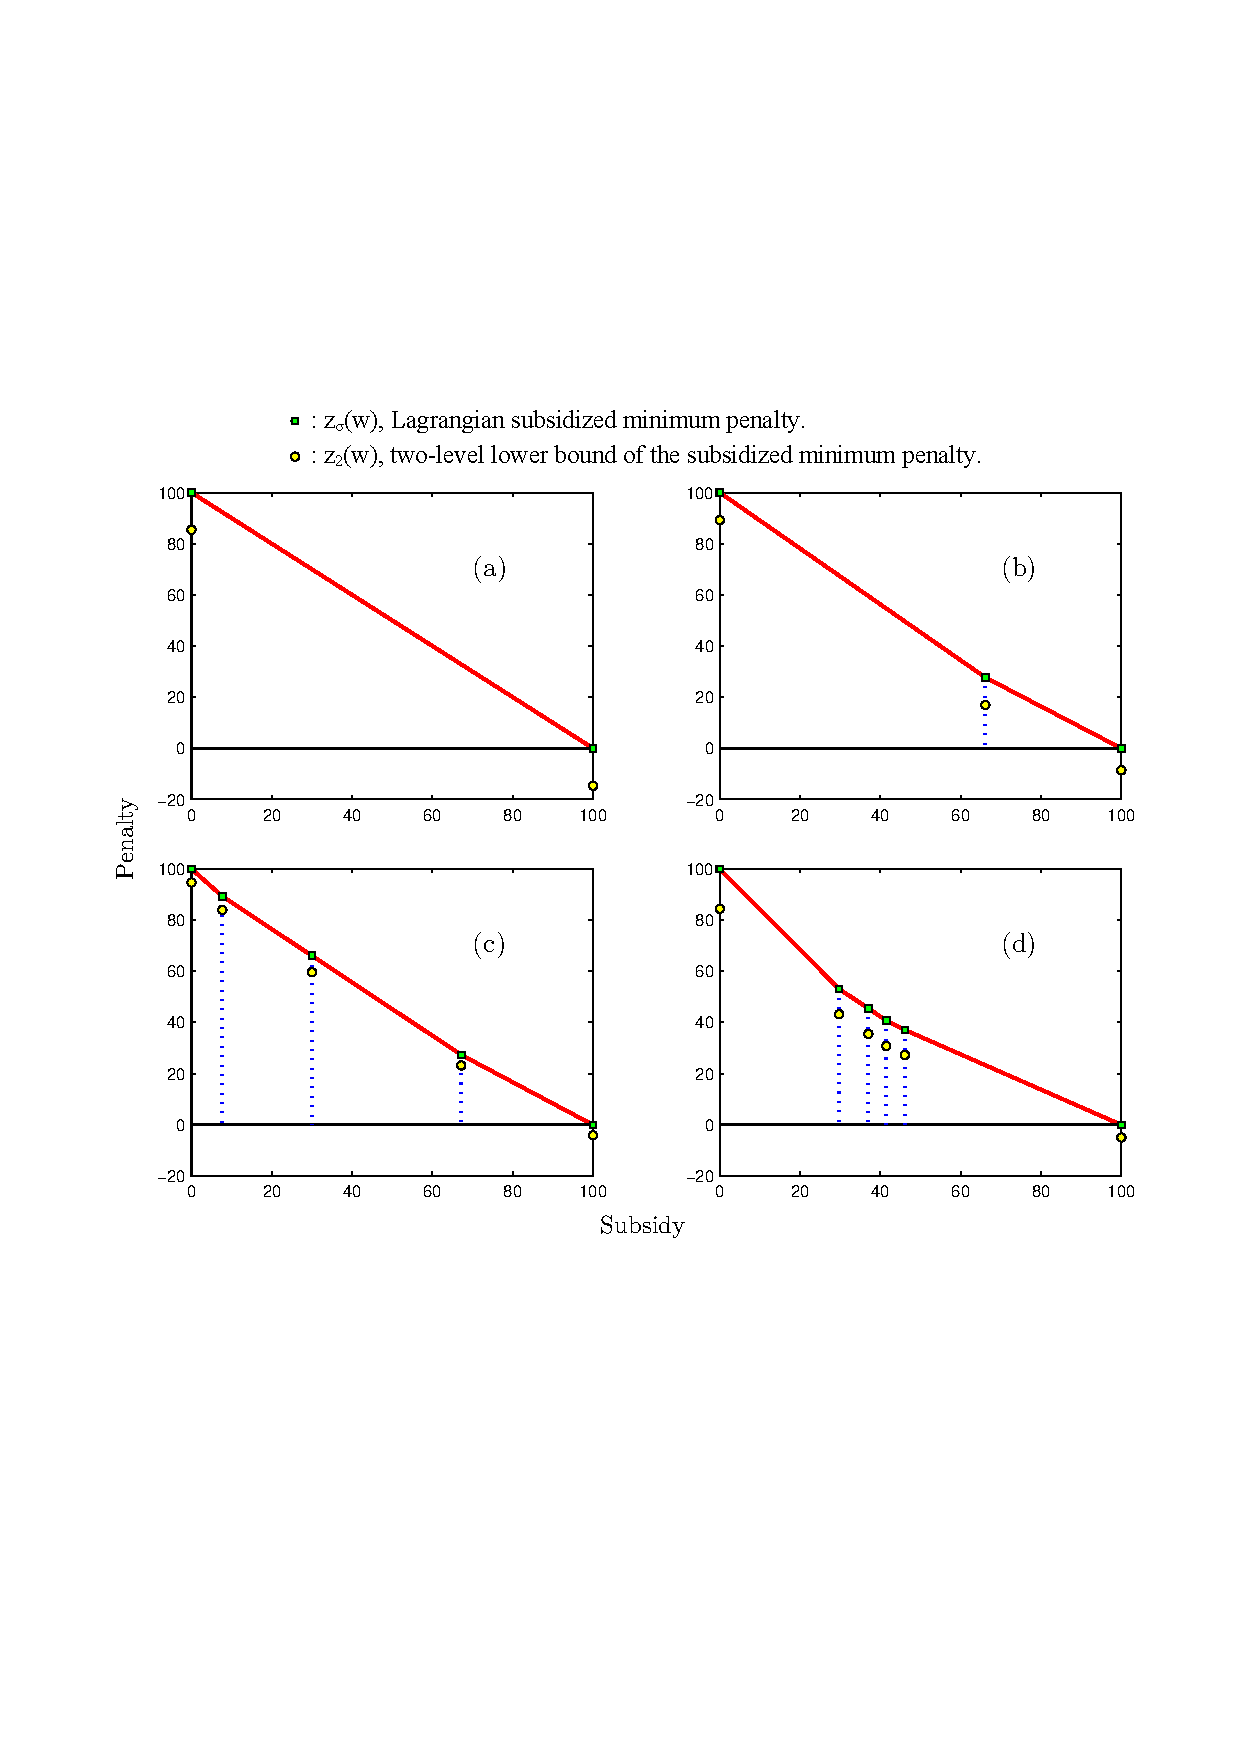
\includegraphics[width=1\textwidth]{1.pdf}
%\captionsetup{font={small}}
\centering
% \caption{\label{figure:20partitioned}Four representative Lagrangian SPFs for TSP games with 20 cities}
\end{figure}
In addition, the meaning of curves (a) and (c) in Figure 2 is explained on page 17.
And the meaning of all curves in Figure 2 are shown below. (a) represents that the respective lines passing the two squared points have the same slope, thus there is no breakpoint between them.
% (a) represents that the slopes at the two points are equal, thus there is no breakpoint between them.
(b) represents that the two lines passing the two squared points at the beginning and the end meets a point, besides, the value of $z_\theta(\omega)$ at x-coordinate value of the point equals the value of y-coordinate of the point which indicates that this point is a breakpoint, which is the middle squared one. (c) represents that the two lines passing the two squared points at the beginning and the end intersects a point under the third squared point. Then with x-coordinate value of this intersection point, the third squared point can be obtained by Algorithm 1 in our manuscript. With the IPC algorithm proposed by Liu et al. (2018), we can generate the line passing the third squared point. Finally, this line intersects the two lines passing the two points at the beginning and the end at the second and fourth squared points, respectively.
% (c) represents that the two lines passing the two points at the beginning and the end meets a point whose y-coordinate value is not equal to the third squared point's y-coordinate value, $z_\theta(\omega)$ at x-coordinate value of the point. The line passing the third squared point intersects the two lines passing the two points at the beginning and the end at the second and fourth squared points, respectively.
The difference of (c) and (d) is that (d) has one more line intersection process than (c) at the right half part of the subfigure.
~\\[4mm]
\noindent \textit{\textbf{Question 10.}
In regards to results of experiments in Table 3, what exactly was used and the upper bound $\phi(N)$? and finally a general remark on the lower bound construction z(w):
-- if we consider problem (4) as a restriction of (2), then it is also possible to create a relaxation of the problem in the similar was as problem (4) was constructed.}
\\[2mm]
\noindent \textbf{Reply 10.}
Thanks for your question. Firstly, the $\phi(N)$ is an upper bound obtained by the Lagrangian relaxation method just like we said in Reply 2.
% The upper bound $\phi(N)$ is what we use Lagrangian heuristic method to obtain.
Secondly, as we mentioned in Reply 1, LP(4) is not a restriction of LP(2). And we know what you thought about the way to create a relaxation of LP(2), we tried this before but it will not work. Thus we designed new methods to obtain the upper and lower bound.

% Based on the above analysis, LP(4) is not a restriction of LP(2), which can also explain why we cannot get a relaxation of LP(2) if we switch the places of $c_l(S)$ and $c_u(S)$ you mentioned in Question 10.
~\\[4mm]

% \noindent \textit{\textbf{Minor comments.}}

% 1. Problem (2) in the paper is frequently called an LP problem or a combinatorial optimization problem (page 4, for example). I suggest to use one terminology approach for consistency. For example, page 8 "solve LP (4) with some conventional combinatorial optimization techniques" sounds confusing.
%
% 2. Remark 1: probably, for any s in S \ V in the first line of the Remark?
%
% 3. Page 8, line 58. Perhaps it is worth mentioning that this is due to Lagrangian being concave function.
%
% 4. Page 10, line 60. Perhaps LP (4) instead of (2)?
%
% 5. Page 10, line 26. Perhaps, it is better to replace forward reference (9) by "reduced cost".
%
% 6. Page 13, I would suggest to make a reference to the Dantzig Fulkerson Johnson (1954) paper with respect to constraints (13), as these constraints are not given in TSP
% literature but are in fact result of development by those authors.
%
% 7. I would suggest merging first two constraints in (11) as it is a bit confusing in its present form.
%
% 8. Page 15, line 45. don't you need to remove the word 'minimum' here?}
%
% \\[2mm]

\noindent \textbf{Reply to Minor Comments.}
Thank you very much for pointing out the errors of our manuscript in Minor comments. We have made the corresponding revisions except the fourth one.

Based on what we demonstrate in Reply 1, LP(4) is not a restriction of LP(2). And what we mean on page 12 is eliminating some constraints of LP(2) to construct a lower bound of the subsidized minimum penalty. Thus, it should be LP(2) on page 12 of the revised manuscript.(Original location is on page 10.)


% 1. We have changed our expression use LP problem to avoid the confusion. according to the Minor comments
%
% 2. We've revised.
%
% 3. We have added the concave property before mentioning the sub-gradient method.

% 5. We've replaced (9) by 'reduced cost' to avoid the forward reference.
%
% 6. We've added a reference to the Dantzig Fulkerson Johnson (1954) paper when introducing constraints (13).
%
% 7. We've merged the first two constraints for the ease of understanding.
%
% 8. We've removed the word 'minimum'.
~\\[4mm]

%\vspace{10mm}
\newpage

\noindent \textbf{\large Reply to Referee 2}
\\[3mm]
Thank you very much for your appreciation.
We have corrected all the typos and grammatical errors that you pointed out.
%As stated in the first two pages, we have made some major changes to the paper structure to strengthen the main contributions of our work.
%Sections 4 and 5 in the original paper are replaced.
%In this report, we will focus on responding to the comments which still mater in the current paper.
%Your other comments will be great helpful in our further study. Thanks a lot for your work.
~\\[4mm]
%
%
%
\noindent \textit{\textbf{Question 1.}
Notation. The paper does not conform with the standard notation in TU-games. Usually, coalitions are referred with capital letters and its cardinal in lower case letters, i.e. $S \subset N$ and $|S| = s$. This paper uses a different notation with $s$ for coalitions and then some inconsistencies appears when referring to $v$ in some places. I would suggest to adapt the notation to the standard to ease the readability of potential readers.}
~\\[2mm]
\noindent \textbf{Reply 1.}
Thanks a lot for your suggestion.
We have changed the notation to the standard form all over the revised manuscript.
\\[4mm]
%
%
%
\noindent \textit{\textbf{Question 2.}
Some confusion appears, here and there, when referring to LP or MIP.
For instance, on page 4 line 3, it is mentioned that (2) is a combinatorial optimization problem. However, (2) is a LP since in its description c is
given and thus all constraints and variables are linear and continuous.
The same confusion can be found at other places of the paper. Please clarify!}
\\[2mm]
\noindent \textbf{Reply 2.}
We have changed our expression with only using LP problem to avoid the confusion.
\\[4mm]
%
%
%
\noindent \textit{\textbf{Question 3.}
Page 4 line -13: The authors must be more precise. The Lagrangean
bound is more accurate than the linear relaxation whenever the problem does not fulfill the integrality property.
}
\\[2mm]
\noindent \textbf{Reply 3.}
Thank you for pointing this out.
We have added this statement, ``for those integer linear programmings which do not fulfill the integrality property", to where you pointed out on page 4.
%We have revised our wordings in line X of page X in the revised manuscript.
\\[4mm]
%
%
%
\noindent \textit{\textbf{Question 4.}
The statement of Theorem 1 should be modified since the value of the
LP is one of the many possible upper bounds not the only one as stated
there.
}
~\\[2mm]
\noindent \textbf{Reply 4.}
This should be ``an". Thanks for pointing this out.
~\\[4mm]
%
%
%
\noindent \textit{\textbf{Question 5.}
Remark 1. The meaning of $v$ is unclear. One should guess that it refers
to $|V|$ but this has to be made explicit.
}
\\[2mm]
\noindent \textbf{Reply 5.}
We have pointed this out in the revised manuscript on page 8.
\\[4mm]
%
%
%
\noindent \textit{\textbf{Question 6.}
Page 8, line -12. Note that (5) is not an LP but an ILP.
}
\\[2mm]
\noindent \textbf{Reply 6.}
Thank you for pointing this out.
This should be ILP.
\\[4mm]
%
%
%
\noindent \textit{\textbf{Question 7.}
To better illustrate the proposed methodology, it would be advisable
to apply it not only to the rooted traveling salesman problem. I would
suggest to add another class of combinatorial games, for instance location games, to the computational study.}
\\[2mm]
\noindent \textbf{Reply 7.}
\textcolor{red}{How to add a computation?}
% Maybe this method applied on another class of combinatorial game is time-consuming and beyond the scope of this manuscript.
\\[4mm]
%
%
%%%%%%%%%%%%%%%%%
\end{document}
%%%%%%%%%%%%%%%%%
